\documentclass[8pt,aspectratio=169]{beamer}
\usetheme{Madrid}
\usepackage{graphicx}
\usepackage{booktabs}
\usepackage{adjustbox}
\usepackage{multicol}
\usepackage{amsmath}
\usepackage{amssymb}
\usepackage{listings}
\usepackage{xcolor}

% Color definitions
\definecolor{mlblue}{RGB}{0,102,204}
\definecolor{mlpurple}{RGB}{51,51,178}
\definecolor{mllavender}{RGB}{173,173,224}
\definecolor{mllavender2}{RGB}{193,193,232}
\definecolor{mllavender3}{RGB}{204,204,235}
\definecolor{mllavender4}{RGB}{214,214,239}
\definecolor{mlorange}{RGB}{255, 127, 14}
\definecolor{mlgreen}{RGB}{44, 160, 44}
\definecolor{mlred}{RGB}{214, 39, 40}
\definecolor{mlgray}{RGB}{127, 127, 127}

% Additional colors for template compatibility
\definecolor{lightgray}{RGB}{240, 240, 240}
\definecolor{midgray}{RGB}{180, 180, 180}

% Solidity colors
\definecolor{solkeyword}{RGB}{0,102,153}
\definecolor{solstring}{RGB}{163,21,21}
\definecolor{solcomment}{RGB}{0,128,0}
\definecolor{solnumber}{RGB}{0,128,128}

% Solidity language definition
\lstdefinelanguage{Solidity}{
  keywords={pragma, solidity, contract, function, public, private, external, internal, view, pure, payable, returns, return, if, else, for, while, mapping, address, uint, uint256, int, string, bool, bytes, bytes32, event, emit, modifier, require, constructor, memory, storage, calldata, msg, sender, value, this, new, delete, true, false},
  keywordstyle=\color{solkeyword}\bfseries,
  sensitive=true,
  comment=[l]{//},
  morecomment=[s]{/*}{*/},
  commentstyle=\color{solcomment}\ttfamily,
  stringstyle=\color{solstring}\ttfamily,
  morestring=[b]',
  morestring=[b]"
}

% Apply custom colors to Madrid theme
\setbeamercolor{palette primary}{bg=mllavender3,fg=mlpurple}
\setbeamercolor{palette secondary}{bg=mllavender2,fg=mlpurple}
\setbeamercolor{palette tertiary}{bg=mllavender,fg=white}
\setbeamercolor{palette quaternary}{bg=mlpurple,fg=white}
\setbeamercolor{structure}{fg=mlpurple}
\setbeamercolor{section in toc}{fg=mlpurple}
\setbeamercolor{subsection in toc}{fg=mlblue}
\setbeamercolor{title}{fg=mlpurple}
\setbeamercolor{frametitle}{fg=mlpurple,bg=mllavender3}
\setbeamercolor{block title}{bg=mllavender2,fg=mlpurple}
\setbeamercolor{block body}{bg=mllavender4,fg=black}

\setbeamertemplate{navigation symbols}{}
\setbeamertemplate{itemize items}[circle]
\setbeamertemplate{enumerate items}[default]
\setbeamersize{text margin left=5mm,text margin right=5mm}

\newcommand{\bottomnote}[1]{%
\vfill
\vspace{-2mm}
\textcolor{mllavender2}{\rule{\textwidth}{0.4pt}}
\vspace{1mm}
\footnotesize
\textbf{#1}
}

% TikZ and pgfplots packages
\usepackage{tikz}
\usepackage{pgfplots}
\pgfplotsset{compat=1.18}
\usetikzlibrary{arrows.meta, positioning, shapes.geometric, shapes.symbols, calc, decorations.pathmorphing, mindmap}

\title{Real-World Assets \& Tokenization: A Visual Introduction}
\subtitle{Standalone Mini-Lecture}
\author{Prof.~Dr.~Joerg Osterrieder}
\institute{University Lecture Series}
\date{\today}
\begin{document}

% Frame 1: Title
\begin{frame}[plain]
\vspace{2cm}
\begin{center}
{\Huge\color{mlpurple} Real-World Assets \& Tokenization: A Visual Introduction}\\[0.4cm]
{\Large\color{mlblue} Standalone Mini-Lecture}\\[0.3cm]
\textcolor{mlgray}{\rule{6cm}{0.4pt}}\\[0.3cm]
{\small\itshape ``Tokenization of real-world assets is the killer app for blockchain'' -- Larry Fink, BlackRock CEO}\\[1.5cm]
{\normalsize Prof.~Dr.~Joerg Osterrieder}\\[0.2cm]
{\small University Lecture Series}\\[0.2cm]
{\small \today}
\end{center}

\bottomnote{This mini-lecture covers tokenization of real-world assets: what it is, asset types, token standards, stablecoins, the Terra collapse, security vs utility tokens, institutional adoption, and the RWA market opportunity.}
\end{frame}

% Frame 2: What is Tokenization?
\begin{frame}{What is Tokenization?}
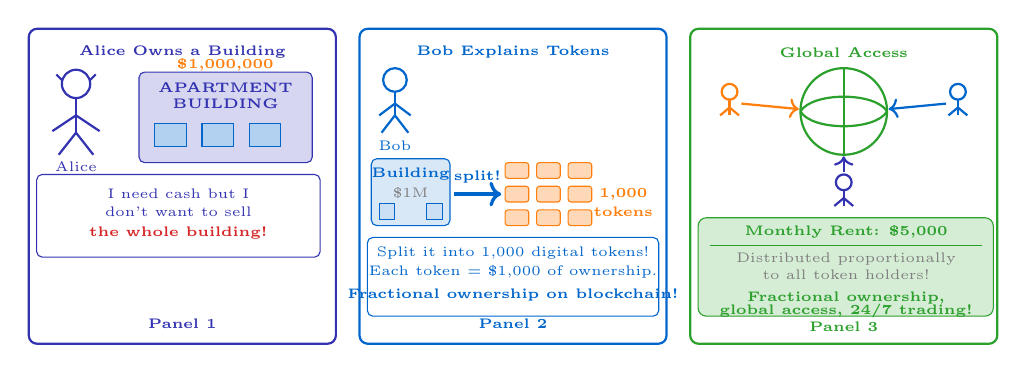
\begin{tikzpicture}
  % Panel borders
  \draw[thick, mlpurple, rounded corners=3pt] (0.1,0.2) rectangle (4.0,4.2);
  \draw[thick, mlblue,   rounded corners=3pt] (4.3,0.2) rectangle (8.2,4.2);
  \draw[thick, mlgreen,  rounded corners=3pt] (8.5,0.2) rectangle (12.4,4.2);

  % --- Panel 1: Alice owns a building ---
  \node[font=\tiny\bfseries, mlpurple] at (2.05,3.9) {Alice Owns a Building};
  % Alice stick figure
  \draw[mlpurple,thick] (0.7,3.5) circle (0.18);
  \draw[mlpurple,thick] (0.7,3.32) -- (0.7,2.88);
  \draw[mlpurple,thick] (0.7,3.1) -- (0.4,2.9);
  \draw[mlpurple,thick] (0.7,3.1) -- (1.0,2.9);
  \draw[mlpurple,thick] (0.7,2.88) -- (0.48,2.60);
  \draw[mlpurple,thick] (0.7,2.88) -- (0.92,2.60);
  \node[font=\tiny, mlpurple] at (0.7,2.45) {Alice};
  % Worried expression lines
  \draw[mlpurple,thick] (0.52,3.55) -- (0.45,3.62);
  \draw[mlpurple,thick] (0.88,3.55) -- (0.95,3.62);
  % Building icon
  \draw[fill=mlpurple!20, draw=mlpurple, rounded corners=2pt] (1.5,2.5) rectangle (3.7,3.65);
  \node[font=\tiny\bfseries, mlpurple, align=center] at (2.6,3.45) {APARTMENT};
  \node[font=\tiny\bfseries, mlpurple, align=center] at (2.6,3.25) {BUILDING};
  % Windows
  \draw[fill=mlblue!30, draw=mlblue] (1.7,2.7) rectangle (2.1,3.0);
  \draw[fill=mlblue!30, draw=mlblue] (2.3,2.7) rectangle (2.7,3.0);
  \draw[fill=mlblue!30, draw=mlblue] (2.9,2.7) rectangle (3.3,3.0);
  % Price tag
  \node[font=\tiny\bfseries, mlorange, align=center] at (2.6,3.75) {\$1,000,000};
  % Speech bubble
  \draw[fill=white, draw=mlpurple, rounded corners=2pt] (0.2,1.3) rectangle (3.8,2.35);
  \node[font=\tiny, mlpurple, align=center] at (2.0,2.1) {I need cash but I};
  \node[font=\tiny, mlpurple, align=center] at (2.0,1.88) {don't want to sell};
  \node[font=\tiny\bfseries, mlred, align=center] at (2.0,1.6) {the whole building!};
  \node[font=\tiny\bfseries, mlpurple] at (2.05,0.45) {Panel 1};

  % --- Panel 2: Bob explains fractionalization ---
  \node[font=\tiny\bfseries, mlblue] at (6.25,3.9) {Bob Explains Tokens};
  % Bob stick figure
  \draw[mlblue,thick] (4.75,3.55) circle (0.15);
  \draw[mlblue,thick] (4.75,3.4) -- (4.75,3.1);
  \draw[mlblue,thick] (4.75,3.25) -- (4.55,3.1);
  \draw[mlblue,thick] (4.75,3.25) -- (4.95,3.1);
  \draw[mlblue,thick] (4.75,3.1) -- (4.58,2.88);
  \draw[mlblue,thick] (4.75,3.1) -- (4.92,2.88);
  \node[font=\tiny, mlblue] at (4.75,2.72) {Bob};
  % Building on left
  \draw[fill=mlblue!15, draw=mlblue, rounded corners=2pt] (4.45,1.7) rectangle (5.45,2.55);
  \node[font=\tiny\bfseries, mlblue, align=center] at (4.95,2.35) {Building};
  \node[font=\tiny, mlgray, align=center] at (4.95,2.12) {\$1M};
  \draw[fill=mlblue!20, draw=mlblue] (4.55,1.78) rectangle (4.75,1.98);
  \draw[fill=mlblue!20, draw=mlblue] (5.15,1.78) rectangle (5.35,1.98);
  % Arrow
  \draw[->, very thick, mlblue] (5.5,2.1) -- (6.1,2.1);
  \node[font=\tiny\bfseries, mlblue, align=center] at (5.8,2.32) {split!};
  % Token grid (3x3 = showing many tokens)
  \draw[fill=mlorange!30, draw=mlorange, rounded corners=1pt] (6.15,2.3) rectangle (6.45,2.5);
  \draw[fill=mlorange!30, draw=mlorange, rounded corners=1pt] (6.55,2.3) rectangle (6.85,2.5);
  \draw[fill=mlorange!30, draw=mlorange, rounded corners=1pt] (6.95,2.3) rectangle (7.25,2.5);
  \draw[fill=mlorange!30, draw=mlorange, rounded corners=1pt] (6.15,2.0) rectangle (6.45,2.2);
  \draw[fill=mlorange!30, draw=mlorange, rounded corners=1pt] (6.55,2.0) rectangle (6.85,2.2);
  \draw[fill=mlorange!30, draw=mlorange, rounded corners=1pt] (6.95,2.0) rectangle (7.25,2.2);
  \draw[fill=mlorange!30, draw=mlorange, rounded corners=1pt] (6.15,1.7) rectangle (6.45,1.9);
  \draw[fill=mlorange!30, draw=mlorange, rounded corners=1pt] (6.55,1.7) rectangle (6.85,1.9);
  \draw[fill=mlorange!30, draw=mlorange, rounded corners=1pt] (6.95,1.7) rectangle (7.25,1.9);
  \node[font=\tiny\bfseries, mlorange, align=center] at (7.65,2.1) {1,000};
  \node[font=\tiny\bfseries, mlorange, align=center] at (7.65,1.88) {tokens};
  % Speech bubble
  \draw[fill=white, draw=mlblue, rounded corners=2pt] (4.4,0.55) rectangle (8.1,1.55);
  \node[font=\tiny, mlblue, align=center] at (6.25,1.35) {Split it into 1,000 digital tokens!};
  \node[font=\tiny, mlblue, align=center] at (6.25,1.12) {Each token = \$1,000 of ownership.};
  \node[font=\tiny\bfseries, mlblue, align=center] at (6.25,0.82) {Fractional ownership on blockchain!};
  \node[font=\tiny\bfseries, mlblue] at (6.25,0.45) {Panel 2};

  % --- Panel 3: Global token trading ---
  \node[font=\tiny\bfseries, mlgreen] at (10.45,3.9) {Global Access};
  % Globe outline
  \draw[mlgreen, thick] (10.45,3.15) circle (0.55);
  \draw[mlgreen, thick] (9.9,3.15) .. controls (10.05,3.4) and (10.85,3.4) .. (11.0,3.15);
  \draw[mlgreen, thick] (9.9,3.15) .. controls (10.05,2.9) and (10.85,2.9) .. (11.0,3.15);
  \draw[mlgreen, thick] (10.45,2.6) -- (10.45,3.7);
  % People around the globe
  \draw[mlorange,thick] (9.0,3.4) circle (0.1);
  \draw[mlorange,thick] (9.0,3.3) -- (9.0,3.1);
  \draw[mlorange,thick] (9.0,3.2) -- (8.88,3.1);
  \draw[mlorange,thick] (9.0,3.2) -- (9.12,3.1);
  \draw[mlblue,thick] (11.9,3.4) circle (0.1);
  \draw[mlblue,thick] (11.9,3.3) -- (11.9,3.1);
  \draw[mlblue,thick] (11.9,3.2) -- (11.78,3.1);
  \draw[mlblue,thick] (11.9,3.2) -- (12.02,3.1);
  \draw[mlpurple,thick] (10.45,2.25) circle (0.1);
  \draw[mlpurple,thick] (10.45,2.15) -- (10.45,1.95);
  \draw[mlpurple,thick] (10.45,2.05) -- (10.33,1.95);
  \draw[mlpurple,thick] (10.45,2.05) -- (10.57,1.95);
  % Arrows to globe (buying tokens)
  \draw[->, thick, mlorange] (9.15,3.25) -- (9.88,3.18);
  \draw[->, thick, mlblue] (11.75,3.25) -- (11.02,3.18);
  \draw[->, thick, mlpurple] (10.45,2.38) -- (10.45,2.58);
  % Rent distribution box
  \draw[fill=mlgreen!20, draw=mlgreen, rounded corners=3pt] (8.6,0.55) rectangle (12.35,1.8);
  \node[font=\tiny\bfseries, mlgreen, align=center] at (10.48,1.62) {Monthly Rent: \$5,000};
  \draw[mlgreen, thin] (8.75,1.45) -- (12.2,1.45);
  \node[font=\tiny, mlgray, align=center] at (10.48,1.28) {Distributed proportionally};
  \node[font=\tiny, mlgray, align=center] at (10.48,1.08) {to all token holders!};
  \node[font=\tiny\bfseries, mlgreen, align=center] at (10.48,0.78) {Fractional ownership,};
  \node[font=\tiny\bfseries, mlgreen, align=center] at (10.48,0.62) {global access, 24/7 trading!};
  \node[font=\tiny\bfseries, mlgreen] at (10.45,0.42) {Panel 3};
\end{tikzpicture}

\bottomnote{Tokenization converts real-world assets into digital blockchain tokens. A \$1M building becomes 1,000 tokens at \$1,000 each -- enabling fractional ownership, global access, and 24/7 trading with automatic income distribution.}
\end{frame}

% Frame 3: Types of Tokenizable Assets
\begin{frame}{Types of Tokenizable Assets}
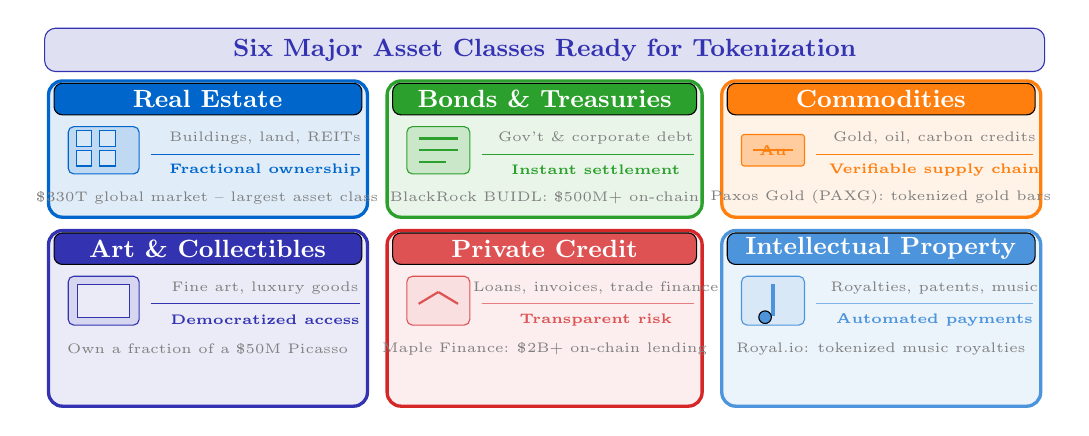
\begin{tikzpicture}
  % Header bar
  \draw[fill=mlpurple!15, draw=mlpurple, rounded corners=4pt] (0.0,4.5) rectangle (12.7,5.05);
  \node[font=\small\bfseries, mlpurple, align=center] at (6.35,4.77) {Six Major Asset Classes Ready for Tokenization};

  % --- Row 1 ---
  % Panel 1: Real Estate
  \draw[fill=mlblue!12, draw=mlblue, very thick, rounded corners=5pt] (0.05,2.65) rectangle (4.1,4.38);
  \draw[fill=mlblue, rounded corners=3pt] (0.12,3.95) rectangle (4.03,4.35);
  \node[font=\small\bfseries, white, align=center] at (2.07,4.15) {Real Estate};
  % Building icon
  \draw[fill=mlblue!25, draw=mlblue, rounded corners=2pt] (0.3,3.2) rectangle (1.2,3.8);
  \draw[fill=mlblue!15, draw=mlblue] (0.4,3.3) rectangle (0.6,3.5);
  \draw[fill=mlblue!15, draw=mlblue] (0.7,3.3) rectangle (0.9,3.5);
  \draw[fill=mlblue!15, draw=mlblue] (0.4,3.55) rectangle (0.6,3.75);
  \draw[fill=mlblue!15, draw=mlblue] (0.7,3.55) rectangle (0.9,3.75);
  \node[font=\tiny, mlgray, align=center] at (2.8,3.65) {Buildings, land, REITs};
  \draw[mlblue, thin] (1.35,3.45) -- (4.0,3.45);
  \node[font=\tiny\bfseries, mlblue, align=center] at (2.8,3.25) {Fractional ownership};
  \node[font=\tiny, mlgray, align=center] at (2.07,2.9) {\$330T global market -- largest asset class};

  % Panel 2: Bonds & Treasuries
  \draw[fill=mlgreen!10, draw=mlgreen, very thick, rounded corners=5pt] (4.35,2.65) rectangle (8.35,4.38);
  \draw[fill=mlgreen, rounded corners=3pt] (4.42,3.95) rectangle (8.28,4.35);
  \node[font=\small\bfseries, white, align=center] at (6.35,4.15) {Bonds \& Treasuries};
  % Document icon
  \draw[fill=mlgreen!25, draw=mlgreen, rounded corners=2pt] (4.6,3.2) rectangle (5.4,3.8);
  \draw[mlgreen, thick] (4.75,3.65) -- (5.25,3.65);
  \draw[mlgreen, thick] (4.75,3.5) -- (5.25,3.5);
  \draw[mlgreen, thick] (4.75,3.35) -- (5.1,3.35);
  \node[font=\tiny, mlgray, align=center] at (7.0,3.65) {Gov't \& corporate debt};
  \draw[mlgreen, thin] (5.55,3.45) -- (8.25,3.45);
  \node[font=\tiny\bfseries, mlgreen, align=center] at (7.0,3.25) {Instant settlement};
  \node[font=\tiny, mlgray, align=center] at (6.35,2.9) {BlackRock BUIDL: \$500M+ on-chain};

  % Panel 3: Commodities
  \draw[fill=mlorange!10, draw=mlorange, very thick, rounded corners=5pt] (8.6,2.65) rectangle (12.65,4.38);
  \draw[fill=mlorange, rounded corners=3pt] (8.67,3.95) rectangle (12.58,4.35);
  \node[font=\small\bfseries, white, align=center] at (10.62,4.15) {Commodities};
  % Gold bar icon
  \draw[fill=mlorange!40, draw=mlorange, rounded corners=1pt] (8.85,3.3) rectangle (9.65,3.7);
  \draw[mlorange, thick] (9.0,3.5) -- (9.5,3.5);
  \node[font=\tiny\bfseries, mlorange, align=center] at (9.25,3.5) {Au};
  \node[font=\tiny, mlgray, align=center] at (11.3,3.65) {Gold, oil, carbon credits};
  \draw[mlorange, thin] (9.8,3.45) -- (12.55,3.45);
  \node[font=\tiny\bfseries, mlorange, align=center] at (11.3,3.25) {Verifiable supply chain};
  \node[font=\tiny, mlgray, align=center] at (10.62,2.9) {Paxos Gold (PAXG): tokenized gold bars};

  % --- Row 2 ---
  % Panel 4: Art & Collectibles
  \draw[fill=mlpurple!10, draw=mlpurple, very thick, rounded corners=5pt] (0.05,0.25) rectangle (4.1,2.48);
  \draw[fill=mlpurple, rounded corners=3pt] (0.12,2.05) rectangle (4.03,2.45);
  \node[font=\small\bfseries, white, align=center] at (2.07,2.25) {Art \& Collectibles};
  % Frame icon
  \draw[fill=mlpurple!20, draw=mlpurple, rounded corners=2pt] (0.3,1.28) rectangle (1.2,1.9);
  \draw[fill=mlpurple!10, draw=mlpurple] (0.42,1.38) rectangle (1.08,1.8);
  \node[font=\tiny, mlgray, align=center] at (2.8,1.75) {Fine art, luxury goods};
  \draw[mlpurple, thin] (1.35,1.55) -- (4.0,1.55);
  \node[font=\tiny\bfseries, mlpurple, align=center] at (2.8,1.35) {Democratized access};
  \node[font=\tiny, mlgray, align=center] at (2.07,0.98) {Own a fraction of a \$50M Picasso};

  % Panel 5: Private Credit
  \draw[fill=mlred!8, draw=mlred, very thick, rounded corners=5pt] (4.35,0.25) rectangle (8.35,2.48);
  \draw[fill=mlred!80, rounded corners=3pt] (4.42,2.05) rectangle (8.28,2.45);
  \node[font=\small\bfseries, white, align=center] at (6.35,2.25) {Private Credit};
  % Handshake icon
  \draw[fill=mlred!15, draw=mlred!80, rounded corners=2pt] (4.6,1.28) rectangle (5.4,1.9);
  \draw[mlred!80, thick] (4.75,1.55) -- (5.0,1.7);
  \draw[mlred!80, thick] (5.0,1.7) -- (5.25,1.55);
  \node[font=\tiny, mlgray, align=center] at (7.0,1.75) {Loans, invoices, trade finance};
  \draw[mlred!60, thin] (5.55,1.55) -- (8.25,1.55);
  \node[font=\tiny\bfseries, mlred!80, align=center] at (7.0,1.35) {Transparent risk};
  \node[font=\tiny, mlgray, align=center] at (6.35,0.98) {Maple Finance: \$2B+ on-chain lending};

  % Panel 6: Intellectual Property
  \draw[fill=mlblue!8, draw=mlblue!70, very thick, rounded corners=5pt] (8.6,0.25) rectangle (12.65,2.48);
  \draw[fill=mlblue!70, rounded corners=3pt] (8.67,2.05) rectangle (12.58,2.45);
  \node[font=\small\bfseries, white, align=center] at (10.62,2.25) {Intellectual Property};
  % Music note icon
  \draw[fill=mlblue!15, draw=mlblue!70, rounded corners=2pt] (8.85,1.28) rectangle (9.65,1.9);
  \draw[mlblue!70, very thick] (9.25,1.4) -- (9.25,1.8);
  \draw[fill=mlblue!70] (9.15,1.38) circle (0.08);
  \node[font=\tiny, mlgray, align=center] at (11.3,1.75) {Royalties, patents, music};
  \draw[mlblue!50, thin] (9.8,1.55) -- (12.55,1.55);
  \node[font=\tiny\bfseries, mlblue!70, align=center] at (11.3,1.35) {Automated payments};
  \node[font=\tiny, mlgray, align=center] at (10.62,0.98) {Royal.io: tokenized music royalties};
\end{tikzpicture}

\bottomnote{Six major asset classes are being tokenized: real estate (\$330T market), bonds (instant settlement), commodities (verifiable), art (democratized), private credit (transparent), and IP (automated royalties).}
\end{frame}

% Frame 4: Token Standards Explained
\begin{frame}{Token Standards Explained}
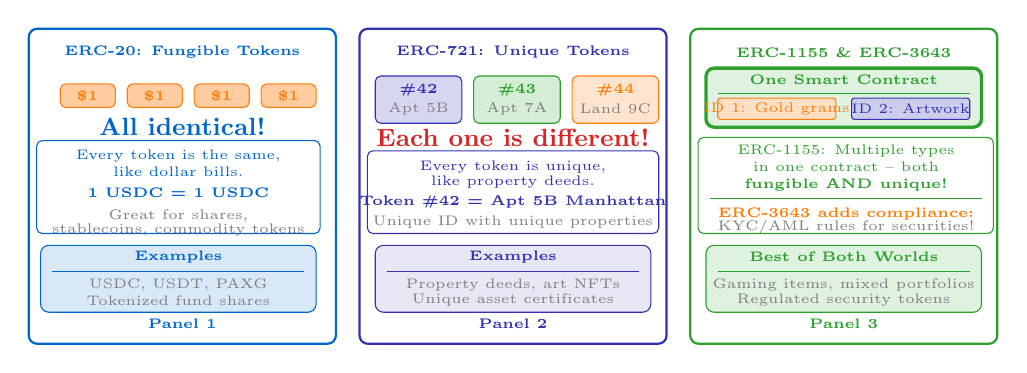
\begin{tikzpicture}
  % Panel borders
  \draw[thick, mlblue,   rounded corners=3pt] (0.1,0.2) rectangle (4.0,4.2);
  \draw[thick, mlpurple, rounded corners=3pt] (4.3,0.2) rectangle (8.2,4.2);
  \draw[thick, mlgreen,  rounded corners=3pt] (8.5,0.2) rectangle (12.4,4.2);

  % --- Panel 1: ERC-20 Fungible ---
  \node[font=\tiny\bfseries, mlblue] at (2.05,3.9) {ERC-20: Fungible Tokens};
  % Stack of identical coins
  \draw[fill=mlorange!40, draw=mlorange, rounded corners=2pt] (0.5,3.2) rectangle (1.2,3.5);
  \node[font=\tiny\bfseries, mlorange, align=center] at (0.85,3.35) {\$1};
  \draw[fill=mlorange!40, draw=mlorange, rounded corners=2pt] (1.35,3.2) rectangle (2.05,3.5);
  \node[font=\tiny\bfseries, mlorange, align=center] at (1.7,3.35) {\$1};
  \draw[fill=mlorange!40, draw=mlorange, rounded corners=2pt] (2.2,3.2) rectangle (2.9,3.5);
  \node[font=\tiny\bfseries, mlorange, align=center] at (2.55,3.35) {\$1};
  \draw[fill=mlorange!40, draw=mlorange, rounded corners=2pt] (3.05,3.2) rectangle (3.75,3.5);
  \node[font=\tiny\bfseries, mlorange, align=center] at (3.4,3.35) {\$1};
  % Equals sign
  \node[font=\small\bfseries, mlblue, align=center] at (2.05,2.95) {All identical!};
  % Speech bubble
  \draw[fill=white, draw=mlblue, rounded corners=2pt] (0.2,1.6) rectangle (3.8,2.78);
  \node[font=\tiny, mlblue, align=center] at (2.0,2.58) {Every token is the same,};
  \node[font=\tiny, mlblue, align=center] at (2.0,2.38) {like dollar bills.};
  \node[font=\tiny\bfseries, mlblue, align=center] at (2.0,2.12) {1 USDC = 1 USDC};
  \node[font=\tiny, mlgray, align=center] at (2.0,1.82) {Great for shares,};
  \node[font=\tiny, mlgray, align=center] at (2.0,1.65) {stablecoins, commodity tokens};
  % Use cases
  \draw[fill=mlblue!15, draw=mlblue, rounded corners=3pt] (0.25,0.6) rectangle (3.75,1.45);
  \node[font=\tiny\bfseries, mlblue, align=center] at (2.0,1.3) {Examples};
  \draw[mlblue, thin] (0.4,1.12) -- (3.6,1.12);
  \node[font=\tiny, mlgray, align=center] at (2.0,0.95) {USDC, USDT, PAXG};
  \node[font=\tiny, mlgray, align=center] at (2.0,0.75) {Tokenized fund shares};
  \node[font=\tiny\bfseries, mlblue] at (2.05,0.45) {Panel 1};

  % --- Panel 2: ERC-721 Unique ---
  \node[font=\tiny\bfseries, mlpurple] at (6.25,3.9) {ERC-721: Unique Tokens};
  % Unique property cards
  \draw[fill=mlpurple!20, draw=mlpurple, rounded corners=2pt] (4.5,3.0) rectangle (5.6,3.6);
  \node[font=\tiny\bfseries, mlpurple, align=center] at (5.05,3.42) {\#42};
  \node[font=\tiny, mlgray, align=center] at (5.05,3.18) {Apt 5B};
  \draw[fill=mlgreen!20, draw=mlgreen, rounded corners=2pt] (5.75,3.0) rectangle (6.85,3.6);
  \node[font=\tiny\bfseries, mlgreen, align=center] at (6.3,3.42) {\#43};
  \node[font=\tiny, mlgray, align=center] at (6.3,3.18) {Apt 7A};
  \draw[fill=mlorange!20, draw=mlorange, rounded corners=2pt] (7.0,3.0) rectangle (8.1,3.6);
  \node[font=\tiny\bfseries, mlorange, align=center] at (7.55,3.42) {\#44};
  \node[font=\tiny, mlgray, align=center] at (7.55,3.18) {Land 9C};
  % Not-equal
  \node[font=\small\bfseries, mlred, align=center] at (6.25,2.82) {Each one is different!};
  % Speech bubble
  \draw[fill=white, draw=mlpurple, rounded corners=2pt] (4.4,1.6) rectangle (8.1,2.65);
  \node[font=\tiny, mlpurple, align=center] at (6.25,2.45) {Every token is unique,};
  \node[font=\tiny, mlpurple, align=center] at (6.25,2.25) {like property deeds.};
  \node[font=\tiny\bfseries, mlpurple, align=center] at (6.25,2.0) {Token \#42 = Apt 5B Manhattan};
  \node[font=\tiny, mlgray, align=center] at (6.25,1.75) {Unique ID with unique properties};
  % Use cases
  \draw[fill=mlpurple!12, draw=mlpurple, rounded corners=3pt] (4.5,0.6) rectangle (8.0,1.45);
  \node[font=\tiny\bfseries, mlpurple, align=center] at (6.25,1.3) {Examples};
  \draw[mlpurple, thin] (4.65,1.12) -- (7.85,1.12);
  \node[font=\tiny, mlgray, align=center] at (6.25,0.95) {Property deeds, art NFTs};
  \node[font=\tiny, mlgray, align=center] at (6.25,0.75) {Unique asset certificates};
  \node[font=\tiny\bfseries, mlpurple] at (6.25,0.45) {Panel 2};

  % --- Panel 3: ERC-1155 & ERC-3643 ---
  \node[font=\tiny\bfseries, mlgreen] at (10.45,3.9) {ERC-1155 \& ERC-3643};
  % Hybrid illustration: fungible + unique from one contract
  \draw[fill=mlgreen!15, draw=mlgreen, very thick, rounded corners=3pt] (8.7,2.95) rectangle (12.2,3.7);
  \node[font=\tiny\bfseries, mlgreen, align=center] at (10.45,3.55) {One Smart Contract};
  \draw[mlgreen, thin] (8.85,3.38) -- (12.05,3.38);
  % Left side: fungible
  \draw[fill=mlorange!25, draw=mlorange, rounded corners=1pt] (8.85,3.05) rectangle (10.35,3.32);
  \node[font=\tiny, mlorange, align=center] at (9.6,3.18) {ID 1: Gold grams};
  % Right side: unique
  \draw[fill=mlpurple!25, draw=mlpurple, rounded corners=1pt] (10.55,3.05) rectangle (12.05,3.32);
  \node[font=\tiny, mlpurple, align=center] at (11.3,3.18) {ID 2: Artwork};
  % Speech bubble
  \draw[fill=white, draw=mlgreen, rounded corners=2pt] (8.6,1.6) rectangle (12.35,2.82);
  \node[font=\tiny, mlgreen, align=center] at (10.48,2.65) {ERC-1155: Multiple types};
  \node[font=\tiny, mlgreen, align=center] at (10.48,2.45) {in one contract -- both};
  \node[font=\tiny\bfseries, mlgreen, align=center] at (10.48,2.22) {fungible AND unique!};
  \draw[mlgreen, thin] (8.75,2.05) -- (12.2,2.05);
  \node[font=\tiny\bfseries, mlorange, align=center] at (10.48,1.85) {ERC-3643 adds compliance:};
  \node[font=\tiny, mlgray, align=center] at (10.48,1.68) {KYC/AML rules for securities!};
  % Bottom box
  \draw[fill=mlgreen!15, draw=mlgreen, rounded corners=3pt] (8.7,0.6) rectangle (12.2,1.45);
  \node[font=\tiny\bfseries, mlgreen, align=center] at (10.45,1.3) {Best of Both Worlds};
  \draw[mlgreen, thin] (8.85,1.12) -- (12.05,1.12);
  \node[font=\tiny, mlgray, align=center] at (10.45,0.95) {Gaming items, mixed portfolios};
  \node[font=\tiny, mlgray, align=center] at (10.45,0.75) {Regulated security tokens};
  \node[font=\tiny\bfseries, mlgreen] at (10.45,0.45) {Panel 3};
\end{tikzpicture}

\bottomnote{ERC-20: fungible tokens (stablecoins, shares). ERC-721: unique tokens (deeds, art). ERC-1155: multi-type (fungible + unique in one contract). ERC-3643: adds compliance rules for regulated security tokens.}
\end{frame}

% Frame 5: Stablecoins: The First Killer App
\begin{frame}{Stablecoins: The First Killer App}
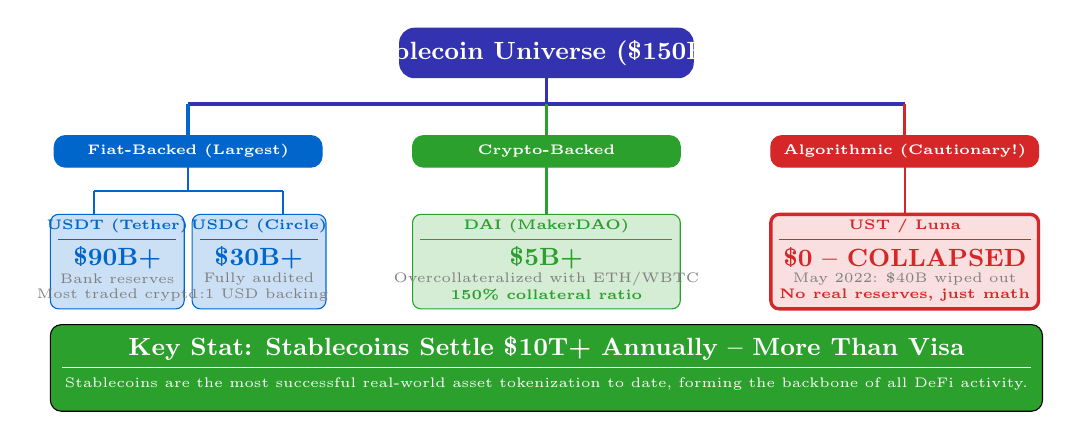
\begin{tikzpicture}
  % Center hub
  \draw[fill=mlpurple, draw=mlpurple, very thick, rounded corners=5pt] (4.5,4.45) rectangle (8.2,5.05);
  \node[font=\small\bfseries, white, align=center] at (6.35,4.75) {Stablecoin Universe (\$150B+)};

  % Root stems
  \draw[very thick, mlpurple] (6.35,4.45) -- (6.35,4.1);
  \draw[very thick, mlpurple] (1.8,4.1) -- (10.9,4.1);

  % --- Branch 1: Fiat-Backed (left) ---
  \draw[very thick, mlblue] (1.8,4.1) -- (1.8,3.7);
  \draw[fill=mlblue, draw=mlblue, rounded corners=4pt] (0.1,3.3) rectangle (3.5,3.7);
  \node[font=\tiny\bfseries, white, align=center] at (1.8,3.5) {Fiat-Backed (Largest)};

  \draw[thick, mlblue] (1.8,3.3) -- (1.8,3.0);
  \draw[thick, mlblue] (0.6,3.0) -- (3.0,3.0);
  \draw[thick, mlblue] (0.6,3.0) -- (0.6,2.7);
  \draw[thick, mlblue] (3.0,3.0) -- (3.0,2.7);

  % USDT box
  \draw[fill=mlblue!20, draw=mlblue, rounded corners=3pt] (0.05,1.5) rectangle (1.75,2.7);
  \node[font=\tiny\bfseries, mlblue, align=center] at (0.9,2.55) {USDT (Tether)};
  \draw[mlblue, thin] (0.15,2.38) -- (1.65,2.38);
  \node[font=\small\bfseries, mlblue, align=center] at (0.9,2.15) {\$90B+};
  \node[font=\tiny, mlgray, align=center] at (0.9,1.88) {Bank reserves};
  \node[font=\tiny, mlgray, align=center] at (0.9,1.68) {Most traded crypto};

  % USDC box
  \draw[fill=mlblue!20, draw=mlblue, rounded corners=3pt] (1.85,1.5) rectangle (3.55,2.7);
  \node[font=\tiny\bfseries, mlblue, align=center] at (2.7,2.55) {USDC (Circle)};
  \draw[mlblue, thin] (1.95,2.38) -- (3.45,2.38);
  \node[font=\small\bfseries, mlblue, align=center] at (2.7,2.15) {\$30B+};
  \node[font=\tiny, mlgray, align=center] at (2.7,1.88) {Fully audited};
  \node[font=\tiny, mlgray, align=center] at (2.7,1.68) {1:1 USD backing};

  % --- Branch 2: Crypto-Backed (center) ---
  \draw[very thick, mlgreen] (6.35,4.1) -- (6.35,3.7);
  \draw[fill=mlgreen, draw=mlgreen, rounded corners=4pt] (4.65,3.3) rectangle (8.05,3.7);
  \node[font=\tiny\bfseries, white, align=center] at (6.35,3.5) {Crypto-Backed};

  \draw[thick, mlgreen] (6.35,3.3) -- (6.35,2.7);

  % DAI box
  \draw[fill=mlgreen!20, draw=mlgreen, rounded corners=3pt] (4.65,1.5) rectangle (8.05,2.7);
  \node[font=\tiny\bfseries, mlgreen, align=center] at (6.35,2.55) {DAI (MakerDAO)};
  \draw[mlgreen, thin] (4.75,2.38) -- (7.95,2.38);
  \node[font=\small\bfseries, mlgreen, align=center] at (6.35,2.15) {\$5B+};
  \node[font=\tiny, mlgray, align=center] at (6.35,1.88) {Overcollateralized with ETH/WBTC};
  \node[font=\tiny\bfseries, mlgreen, align=center] at (6.35,1.68) {150\% collateral ratio};

  % --- Branch 3: Algorithmic (right) ---
  \draw[very thick, mlred] (10.9,4.1) -- (10.9,3.7);
  \draw[fill=mlred, draw=mlred, rounded corners=4pt] (9.2,3.3) rectangle (12.6,3.7);
  \node[font=\tiny\bfseries, white, align=center] at (10.9,3.5) {Algorithmic (Cautionary!)};

  \draw[thick, mlred] (10.9,3.3) -- (10.9,2.7);

  % UST box with skull
  \draw[fill=mlred!15, draw=mlred, very thick, rounded corners=3pt] (9.2,1.5) rectangle (12.6,2.7);
  \node[font=\tiny\bfseries, mlred, align=center] at (10.9,2.55) {UST / Luna};
  \draw[mlred, thin] (9.3,2.38) -- (12.5,2.38);
  \node[font=\small\bfseries, mlred, align=center] at (10.9,2.15) {\$0 -- COLLAPSED};
  \node[font=\tiny, mlgray, align=center] at (10.9,1.88) {May 2022: \$40B wiped out};
  \node[font=\tiny\bfseries, mlred, align=center] at (10.9,1.68) {No real reserves, just math};

  % Bottom stat bar
  \draw[fill=mlgreen, rounded corners=4pt] (0.05,0.2) rectangle (12.65,1.3);
  \node[font=\small\bfseries, white, align=center] at (6.35,1.0) {Key Stat: Stablecoins Settle \$10T+ Annually -- More Than Visa};
  \draw[white, thin] (0.2,0.75) -- (12.5,0.75);
  \node[font=\tiny, white, align=center] at (6.35,0.55) {Stablecoins are the most successful real-world asset tokenization to date, forming the backbone of all DeFi activity.};
\end{tikzpicture}

\bottomnote{Stablecoins (\$150B+ market cap) are the first killer app of tokenization. Fiat-backed (USDT, USDC) dominate. Crypto-backed (DAI) use overcollateralization. Algorithmic (UST) collapsed spectacularly. Stablecoins settle more value annually than Visa.}
\end{frame}

% Frame 6: The Terra/Luna Collapse
\begin{frame}{The Terra/Luna Collapse}
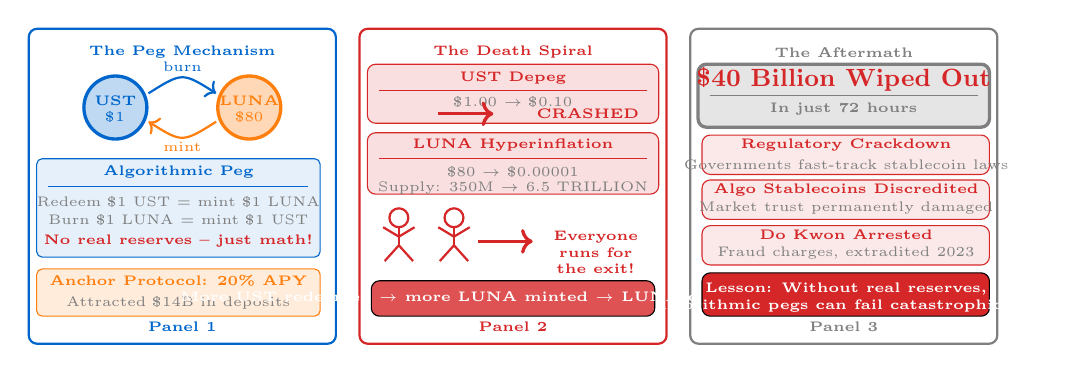
\begin{tikzpicture}
  % Panel borders
  \draw[thick, mlblue,   rounded corners=3pt] (0.1,0.2) rectangle (4.0,4.2);
  \draw[thick, mlred,    rounded corners=3pt] (4.3,0.2) rectangle (8.2,4.2);
  \draw[thick, mlgray,   rounded corners=3pt] (8.5,0.2) rectangle (12.4,4.2);

  % --- Panel 1: The Peg Mechanism ---
  \node[font=\tiny\bfseries, mlblue] at (2.05,3.9) {The Peg Mechanism};
  % UST circle
  \draw[fill=mlblue!25, draw=mlblue, very thick] (1.2,3.2) circle (0.4);
  \node[font=\tiny\bfseries, mlblue, align=center] at (1.2,3.28) {UST};
  \node[font=\tiny, mlblue, align=center] at (1.2,3.08) {\$1};
  % LUNA circle
  \draw[fill=mlorange!30, draw=mlorange, very thick] (2.9,3.2) circle (0.4);
  \node[font=\tiny\bfseries, mlorange, align=center] at (2.9,3.28) {LUNA};
  \node[font=\tiny, mlorange, align=center] at (2.9,3.08) {\$80};
  % Circular arrows between them
  \draw[->, thick, mlblue] (1.62,3.38) .. controls (2.05,3.65) .. (2.48,3.38);
  \node[font=\tiny, mlblue, align=center] at (2.05,3.72) {burn};
  \draw[->, thick, mlorange] (2.48,3.02) .. controls (2.05,2.75) .. (1.62,3.02);
  \node[font=\tiny, mlorange, align=center] at (2.05,2.7) {mint};
  % Explanation
  \draw[fill=mlblue!10, draw=mlblue, rounded corners=2pt] (0.2,1.3) rectangle (3.8,2.55);
  \node[font=\tiny\bfseries, mlblue, align=center] at (2.0,2.38) {Algorithmic Peg};
  \draw[mlblue, thin] (0.35,2.2) -- (3.65,2.2);
  \node[font=\tiny, mlgray, align=center] at (2.0,2.0) {Redeem \$1 UST = mint \$1 LUNA};
  \node[font=\tiny, mlgray, align=center] at (2.0,1.78) {Burn \$1 LUNA = mint \$1 UST};
  \node[font=\tiny\bfseries, mlred, align=center] at (2.0,1.5) {No real reserves -- just math!};
  % Anchor protocol
  \draw[fill=mlorange!15, draw=mlorange, rounded corners=2pt] (0.2,0.55) rectangle (3.8,1.15);
  \node[font=\tiny\bfseries, mlorange, align=center] at (2.0,1.0) {Anchor Protocol: 20\% APY};
  \node[font=\tiny, mlgray, align=center] at (2.0,0.72) {Attracted \$14B in deposits};
  \node[font=\tiny\bfseries, mlblue] at (2.05,0.42) {Panel 1};

  % --- Panel 2: The Death Spiral ---
  \node[font=\tiny\bfseries, mlred] at (6.25,3.9) {The Death Spiral};
  % UST depeg arrow
  \draw[fill=mlred!15, draw=mlred, rounded corners=3pt] (4.4,3.0) rectangle (8.1,3.75);
  \node[font=\tiny\bfseries, mlred, align=center] at (6.25,3.58) {UST Depeg};
  \draw[mlred, thin] (4.55,3.42) -- (7.95,3.42);
  \node[font=\tiny, mlgray, align=center] at (6.25,3.28) {\$1.00 $\to$ \$0.10};
  \draw[->, very thick, mlred] (5.3,3.12) -- (6.0,3.12);
  \node[font=\tiny\bfseries, mlred, align=center] at (7.2,3.12) {CRASHED};
  % LUNA hyperinflation
  \draw[fill=mlred!15, draw=mlred, rounded corners=3pt] (4.4,2.1) rectangle (8.1,2.88);
  \node[font=\tiny\bfseries, mlred, align=center] at (6.25,2.72) {LUNA Hyperinflation};
  \draw[mlred, thin] (4.55,2.55) -- (7.95,2.55);
  \node[font=\tiny, mlgray, align=center] at (6.25,2.38) {\$80 $\to$ \$0.00001};
  \node[font=\tiny, mlgray, align=center] at (6.25,2.18) {Supply: 350M $\to$ 6.5 TRILLION};
  % Panicked stick figures
  \draw[mlred,thick] (4.8,1.8) circle (0.12);
  \draw[mlred,thick] (4.8,1.68) -- (4.8,1.45);
  \draw[mlred,thick] (4.8,1.56) -- (4.6,1.68);
  \draw[mlred,thick] (4.8,1.56) -- (5.0,1.68);
  \draw[mlred,thick] (4.8,1.45) -- (4.62,1.25);
  \draw[mlred,thick] (4.8,1.45) -- (4.98,1.25);
  \draw[mlred,thick] (5.5,1.8) circle (0.12);
  \draw[mlred,thick] (5.5,1.68) -- (5.5,1.45);
  \draw[mlred,thick] (5.5,1.56) -- (5.3,1.68);
  \draw[mlred,thick] (5.5,1.56) -- (5.7,1.68);
  \draw[mlred,thick] (5.5,1.45) -- (5.32,1.25);
  \draw[mlred,thick] (5.5,1.45) -- (5.68,1.25);
  \draw[->, very thick, mlred] (5.8,1.5) -- (6.5,1.5);
  \node[font=\tiny\bfseries, mlred, align=center] at (7.3,1.55) {Everyone};
  \node[font=\tiny\bfseries, mlred, align=center] at (7.3,1.35) {runs for};
  \node[font=\tiny\bfseries, mlred, align=center] at (7.3,1.15) {the exit!};
  % Bottom label
  \draw[fill=mlred!80, rounded corners=3pt] (4.45,0.55) rectangle (8.05,1.0);
  \node[font=\tiny\bfseries, white, align=center] at (6.25,0.78) {More UST redeemed $\to$ more LUNA minted $\to$ LUNA crashes $\to$ repeat};
  \node[font=\tiny\bfseries, mlred] at (6.25,0.42) {Panel 2};

  % --- Panel 3: The Aftermath ---
  \node[font=\tiny\bfseries, mlgray] at (10.45,3.9) {The Aftermath};
  % Newspaper headline style
  \draw[fill=mlgray!20, draw=mlgray, very thick, rounded corners=3pt] (8.6,2.95) rectangle (12.3,3.75);
  \node[font=\small\bfseries, mlred, align=center] at (10.45,3.55) {\$40 Billion Wiped Out};
  \draw[mlgray, thin] (8.75,3.35) -- (12.15,3.35);
  \node[font=\tiny\bfseries, mlgray, align=center] at (10.45,3.18) {In just 72 hours};

  % Consequences
  \draw[fill=mlred!10, draw=mlred, rounded corners=3pt] (8.65,2.35) rectangle (12.3,2.85);
  \node[font=\tiny\bfseries, mlred, align=center] at (10.48,2.72) {Regulatory Crackdown};
  \node[font=\tiny, mlgray, align=center] at (10.48,2.48) {Governments fast-track stablecoin laws};

  \draw[fill=mlred!10, draw=mlred, rounded corners=3pt] (8.65,1.78) rectangle (12.3,2.28);
  \node[font=\tiny\bfseries, mlred, align=center] at (10.48,2.15) {Algo Stablecoins Discredited};
  \node[font=\tiny, mlgray, align=center] at (10.48,1.92) {Market trust permanently damaged};

  \draw[fill=mlred!10, draw=mlred, rounded corners=3pt] (8.65,1.2) rectangle (12.3,1.7);
  \node[font=\tiny\bfseries, mlred, align=center] at (10.48,1.58) {Do Kwon Arrested};
  \node[font=\tiny, mlgray, align=center] at (10.48,1.35) {Fraud charges, extradited 2023};

  % Lesson box
  \draw[fill=mlred, rounded corners=3pt] (8.65,0.55) rectangle (12.3,1.1);
  \node[font=\tiny\bfseries, white, align=center] at (10.48,0.9) {Lesson: Without real reserves,};
  \node[font=\tiny\bfseries, white, align=center] at (10.48,0.68) {algorithmic pegs can fail catastrophically};
  \node[font=\tiny\bfseries, mlgray] at (10.45,0.42) {Panel 3};
\end{tikzpicture}

\bottomnote{The Terra/Luna collapse (May 2022) destroyed \$40B in 72 hours. UST's algorithmic peg failed in a death spiral: mass redemptions hyperinflated LUNA from \$80 to near zero. This was the largest crypto collapse in history.}
\end{frame}

% Frame 7: Security Tokens vs Utility Tokens
\begin{frame}{Security Tokens vs.\ Utility Tokens}
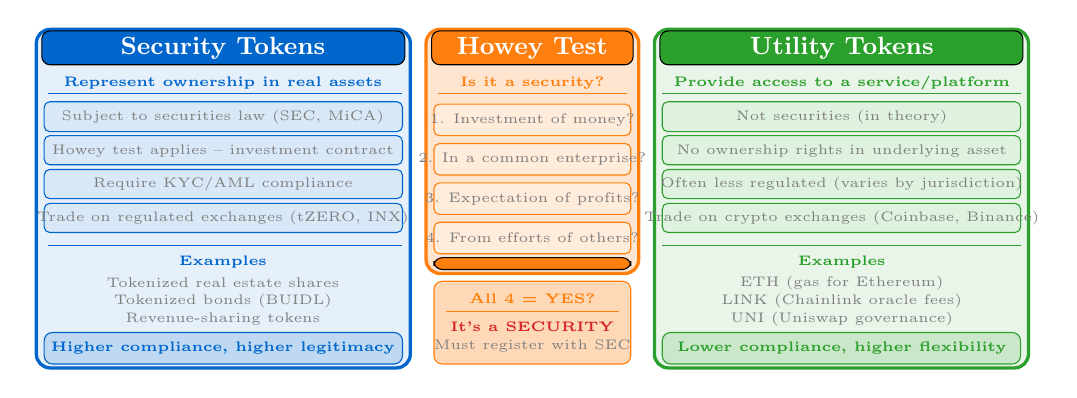
\begin{tikzpicture}
  % --- Left: Security Tokens ---
  \draw[fill=mlblue!10, draw=mlblue, very thick, rounded corners=5pt] (0.05,0.6) rectangle (4.8,4.9);
  \draw[fill=mlblue, rounded corners=3pt] (0.12,4.45) rectangle (4.73,4.88);
  \node[font=\small\bfseries, white, align=center] at (2.42,4.66) {Security Tokens};

  \node[font=\tiny\bfseries, mlblue, align=center] at (2.42,4.22) {Represent ownership in real assets};
  \draw[mlblue, thin] (0.2,4.08) -- (4.7,4.08);

  \draw[fill=mlblue!15, draw=mlblue, rounded corners=2pt] (0.15,3.6) rectangle (4.7,3.98);
  \node[font=\tiny, mlgray, align=center] at (2.42,3.79) {Subject to securities law (SEC, MiCA)};

  \draw[fill=mlblue!15, draw=mlblue, rounded corners=2pt] (0.15,3.18) rectangle (4.7,3.55);
  \node[font=\tiny, mlgray, align=center] at (2.42,3.36) {Howey test applies -- investment contract};

  \draw[fill=mlblue!15, draw=mlblue, rounded corners=2pt] (0.15,2.75) rectangle (4.7,3.12);
  \node[font=\tiny, mlgray, align=center] at (2.42,2.93) {Require KYC/AML compliance};

  \draw[fill=mlblue!15, draw=mlblue, rounded corners=2pt] (0.15,2.32) rectangle (4.7,2.69);
  \node[font=\tiny, mlgray, align=center] at (2.42,2.5) {Trade on regulated exchanges (tZERO, INX)};

  \draw[mlblue, thin] (0.2,2.15) -- (4.7,2.15);
  \node[font=\tiny\bfseries, mlblue, align=center] at (2.42,1.95) {Examples};
  \node[font=\tiny, mlgray, align=center] at (2.42,1.68) {Tokenized real estate shares};
  \node[font=\tiny, mlgray, align=center] at (2.42,1.45) {Tokenized bonds (BUIDL)};
  \node[font=\tiny, mlgray, align=center] at (2.42,1.22) {Revenue-sharing tokens};

  \draw[fill=mlblue!25, draw=mlblue, rounded corners=3pt] (0.15,0.65) rectangle (4.7,1.05);
  \node[font=\tiny\bfseries, mlblue, align=center] at (2.42,0.85) {Higher compliance, higher legitimacy};

  % --- Center: Howey Test ---
  \draw[fill=mlorange!20, draw=mlorange, very thick, rounded corners=5pt] (5.0,1.8) rectangle (7.7,4.9);
  \draw[fill=mlorange, rounded corners=3pt] (5.07,4.45) rectangle (7.63,4.88);
  \node[font=\small\bfseries, white, align=center] at (6.35,4.66) {Howey Test};

  \node[font=\tiny\bfseries, mlorange, align=center] at (6.35,4.22) {Is it a security?};
  \draw[mlorange, thin] (5.15,4.08) -- (7.55,4.08);

  \draw[fill=mlorange!15, draw=mlorange, rounded corners=2pt] (5.1,3.55) rectangle (7.6,3.95);
  \node[font=\tiny, mlgray, align=center] at (6.35,3.75) {1. Investment of money?};

  \draw[fill=mlorange!15, draw=mlorange, rounded corners=2pt] (5.1,3.05) rectangle (7.6,3.45);
  \node[font=\tiny, mlgray, align=center] at (6.35,3.25) {2. In a common enterprise?};

  \draw[fill=mlorange!15, draw=mlorange, rounded corners=2pt] (5.1,2.55) rectangle (7.6,2.95);
  \node[font=\tiny, mlgray, align=center] at (6.35,2.75) {3. Expectation of profits?};

  \draw[fill=mlorange!15, draw=mlorange, rounded corners=2pt] (5.1,2.05) rectangle (7.6,2.45);
  \node[font=\tiny, mlgray, align=center] at (6.35,2.25) {4. From efforts of others?};

  \draw[fill=mlorange, rounded corners=3pt] (5.1,1.85) rectangle (7.6,2.0);

  % Bottom center box
  \draw[fill=mlorange!30, draw=mlorange, rounded corners=3pt] (5.1,0.65) rectangle (7.6,1.7);
  \node[font=\tiny\bfseries, mlorange, align=center] at (6.35,1.48) {All 4 = YES?};
  \draw[mlorange, thin] (5.25,1.32) -- (7.45,1.32);
  \node[font=\tiny\bfseries, mlred, align=center] at (6.35,1.12) {It's a SECURITY};
  \node[font=\tiny, mlgray, align=center] at (6.35,0.88) {Must register with SEC};

  % --- Right: Utility Tokens ---
  \draw[fill=mlgreen!10, draw=mlgreen, very thick, rounded corners=5pt] (7.9,0.6) rectangle (12.65,4.9);
  \draw[fill=mlgreen, rounded corners=3pt] (7.97,4.45) rectangle (12.58,4.88);
  \node[font=\small\bfseries, white, align=center] at (10.28,4.66) {Utility Tokens};

  \node[font=\tiny\bfseries, mlgreen, align=center] at (10.28,4.22) {Provide access to a service/platform};
  \draw[mlgreen, thin] (8.0,4.08) -- (12.55,4.08);

  \draw[fill=mlgreen!15, draw=mlgreen, rounded corners=2pt] (8.0,3.6) rectangle (12.55,3.98);
  \node[font=\tiny, mlgray, align=center] at (10.28,3.79) {Not securities (in theory)};

  \draw[fill=mlgreen!15, draw=mlgreen, rounded corners=2pt] (8.0,3.18) rectangle (12.55,3.55);
  \node[font=\tiny, mlgray, align=center] at (10.28,3.36) {No ownership rights in underlying asset};

  \draw[fill=mlgreen!15, draw=mlgreen, rounded corners=2pt] (8.0,2.75) rectangle (12.55,3.12);
  \node[font=\tiny, mlgray, align=center] at (10.28,2.93) {Often less regulated (varies by jurisdiction)};

  \draw[fill=mlgreen!15, draw=mlgreen, rounded corners=2pt] (8.0,2.32) rectangle (12.55,2.69);
  \node[font=\tiny, mlgray, align=center] at (10.28,2.5) {Trade on crypto exchanges (Coinbase, Binance)};

  \draw[mlgreen, thin] (8.0,2.15) -- (12.55,2.15);
  \node[font=\tiny\bfseries, mlgreen, align=center] at (10.28,1.95) {Examples};
  \node[font=\tiny, mlgray, align=center] at (10.28,1.68) {ETH (gas for Ethereum)};
  \node[font=\tiny, mlgray, align=center] at (10.28,1.45) {LINK (Chainlink oracle fees)};
  \node[font=\tiny, mlgray, align=center] at (10.28,1.22) {UNI (Uniswap governance)};

  \draw[fill=mlgreen!25, draw=mlgreen, rounded corners=3pt] (8.0,0.65) rectangle (12.55,1.05);
  \node[font=\tiny\bfseries, mlgreen, align=center] at (10.28,0.85) {Lower compliance, higher flexibility};
\end{tikzpicture}

\bottomnote{Security tokens represent ownership and must comply with securities law (Howey test, KYC/AML). Utility tokens provide platform access and face less regulation. The Howey test determines classification: investment + common enterprise + expected profits + from others' efforts = security.}
\end{frame}

% Frame 8: BlackRock & Institutional Adoption
\begin{frame}{BlackRock \& Institutional Adoption}
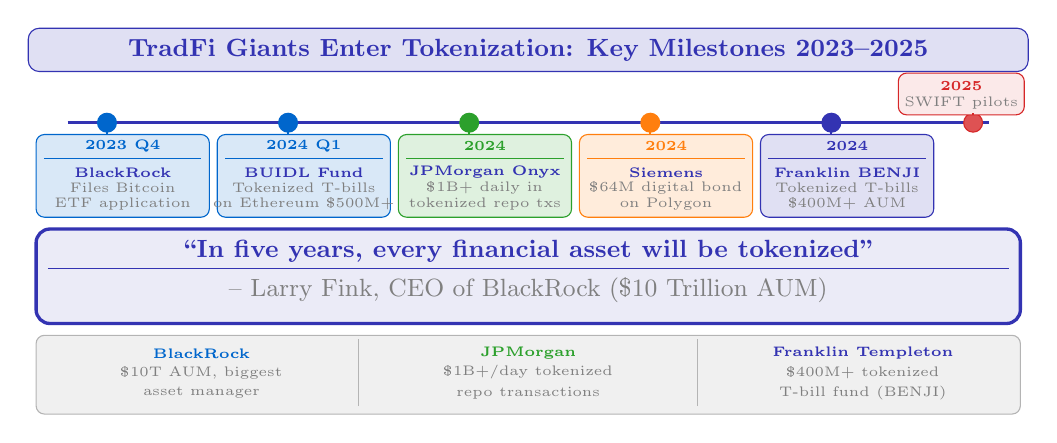
\begin{tikzpicture}
  % Header
  \draw[fill=mlpurple!15, draw=mlpurple, rounded corners=4pt] (0.0,4.5) rectangle (12.7,5.05);
  \node[font=\small\bfseries, mlpurple, align=center] at (6.35,4.77) {TradFi Giants Enter Tokenization: Key Milestones 2023--2025};

  % Timeline line
  \draw[very thick, mlpurple] (0.5,3.85) -- (12.2,3.85);

  % Timeline dots and events
  % Event 1: 2023 Q4
  \draw[fill=mlblue, draw=mlblue] (1.0,3.85) circle (0.12);
  \draw[fill=mlblue!15, draw=mlblue, rounded corners=3pt] (0.1,2.65) rectangle (2.3,3.7);
  \draw[thick, mlblue] (1.0,3.73) -- (1.0,3.7);
  \node[font=\tiny\bfseries, mlblue, align=center] at (1.2,3.55) {2023 Q4};
  \draw[mlblue, thin] (0.2,3.4) -- (2.2,3.4);
  \node[font=\tiny\bfseries, mlpurple, align=center] at (1.2,3.22) {BlackRock};
  \node[font=\tiny, mlgray, align=center] at (1.2,3.02) {Files Bitcoin};
  \node[font=\tiny, mlgray, align=center] at (1.2,2.82) {ETF application};

  % Event 2: 2024 Q1
  \draw[fill=mlblue, draw=mlblue] (3.3,3.85) circle (0.12);
  \draw[fill=mlblue!15, draw=mlblue, rounded corners=3pt] (2.4,2.65) rectangle (4.6,3.7);
  \draw[thick, mlblue] (3.3,3.73) -- (3.3,3.7);
  \node[font=\tiny\bfseries, mlblue, align=center] at (3.5,3.55) {2024 Q1};
  \draw[mlblue, thin] (2.5,3.4) -- (4.5,3.4);
  \node[font=\tiny\bfseries, mlpurple, align=center] at (3.5,3.22) {BUIDL Fund};
  \node[font=\tiny, mlgray, align=center] at (3.5,3.02) {Tokenized T-bills};
  \node[font=\tiny, mlgray, align=center] at (3.5,2.82) {on Ethereum \$500M+};

  % Event 3: 2024
  \draw[fill=mlgreen, draw=mlgreen] (5.6,3.85) circle (0.12);
  \draw[fill=mlgreen!15, draw=mlgreen, rounded corners=3pt] (4.7,2.65) rectangle (6.9,3.7);
  \draw[thick, mlgreen] (5.6,3.73) -- (5.6,3.7);
  \node[font=\tiny\bfseries, mlgreen, align=center] at (5.8,3.55) {2024};
  \draw[mlgreen, thin] (4.8,3.4) -- (6.8,3.4);
  \node[font=\tiny\bfseries, mlpurple, align=center] at (5.8,3.22) {JPMorgan Onyx};
  \node[font=\tiny, mlgray, align=center] at (5.8,3.02) {\$1B+ daily in};
  \node[font=\tiny, mlgray, align=center] at (5.8,2.82) {tokenized repo txs};

  % Event 4: 2024
  \draw[fill=mlorange, draw=mlorange] (7.9,3.85) circle (0.12);
  \draw[fill=mlorange!15, draw=mlorange, rounded corners=3pt] (7.0,2.65) rectangle (9.2,3.7);
  \draw[thick, mlorange] (7.9,3.73) -- (7.9,3.7);
  \node[font=\tiny\bfseries, mlorange, align=center] at (8.1,3.55) {2024};
  \draw[mlorange, thin] (7.1,3.4) -- (9.1,3.4);
  \node[font=\tiny\bfseries, mlpurple, align=center] at (8.1,3.22) {Siemens};
  \node[font=\tiny, mlgray, align=center] at (8.1,3.02) {\$64M digital bond};
  \node[font=\tiny, mlgray, align=center] at (8.1,2.82) {on Polygon};

  % Event 5: 2024
  \draw[fill=mlpurple, draw=mlpurple] (10.2,3.85) circle (0.12);
  \draw[fill=mlpurple!15, draw=mlpurple, rounded corners=3pt] (9.3,2.65) rectangle (11.5,3.7);
  \draw[thick, mlpurple] (10.2,3.73) -- (10.2,3.7);
  \node[font=\tiny\bfseries, mlpurple, align=center] at (10.4,3.55) {2024};
  \draw[mlpurple, thin] (9.4,3.4) -- (11.4,3.4);
  \node[font=\tiny\bfseries, mlpurple, align=center] at (10.4,3.22) {Franklin BENJI};
  \node[font=\tiny, mlgray, align=center] at (10.4,3.02) {Tokenized T-bills};
  \node[font=\tiny, mlgray, align=center] at (10.4,2.82) {\$400M+ AUM};

  % Event 6: 2025
  \draw[fill=mlred!80, draw=mlred] (12.0,3.85) circle (0.12);
  \draw[fill=mlred!10, draw=mlred, rounded corners=3pt] (11.05,3.95) rectangle (12.65,4.48);
  \draw[thick, mlred] (12.0,3.97) -- (12.0,3.95);
  \node[font=\tiny\bfseries, mlred, align=center] at (11.85,4.32) {2025};
  \node[font=\tiny, mlgray, align=center] at (11.85,4.1) {SWIFT pilots};

  % Larry Fink quote box
  \draw[fill=mlpurple!10, draw=mlpurple, very thick, rounded corners=5pt] (0.1,1.3) rectangle (12.6,2.5);
  \node[font=\small\bfseries, mlpurple, align=center] at (6.35,2.22) {``In five years, every financial asset will be tokenized''};
  \draw[mlpurple, thin] (0.25,2.0) -- (12.45,2.0);
  \node[font=\small, mlgray, align=center] at (6.35,1.72) {-- Larry Fink, CEO of BlackRock (\$10 Trillion AUM)};

  % Bottom bar
  \draw[fill=lightgray, draw=midgray, rounded corners=3pt] (0.1,0.15) rectangle (12.6,1.15);
  \node[font=\tiny\bfseries, mlblue, align=center] at (2.2,0.92) {BlackRock};
  \node[font=\tiny, mlgray, align=center] at (2.2,0.68) {\$10T AUM, biggest};
  \node[font=\tiny, mlgray, align=center] at (2.2,0.42) {asset manager};
  \draw[midgray, thin] (4.2,0.25) -- (4.2,1.1);
  \node[font=\tiny\bfseries, mlgreen, align=center] at (6.35,0.92) {JPMorgan};
  \node[font=\tiny, mlgray, align=center] at (6.35,0.68) {\$1B+/day tokenized};
  \node[font=\tiny, mlgray, align=center] at (6.35,0.42) {repo transactions};
  \draw[midgray, thin] (8.5,0.25) -- (8.5,1.1);
  \node[font=\tiny\bfseries, mlpurple, align=center] at (10.6,0.92) {Franklin Templeton};
  \node[font=\tiny, mlgray, align=center] at (10.6,0.68) {\$400M+ tokenized};
  \node[font=\tiny, mlgray, align=center] at (10.6,0.42) {T-bill fund (BENJI)};
\end{tikzpicture}

\bottomnote{The world's largest financial institutions are actively tokenizing assets. BlackRock's BUIDL fund, JPMorgan Onyx, Siemens digital bonds, and Franklin Templeton BENJI demonstrate that tokenization has moved from concept to institutional reality.}
\end{frame}

% Frame 9: The RWA Market Opportunity
\begin{frame}{The RWA Market Opportunity}
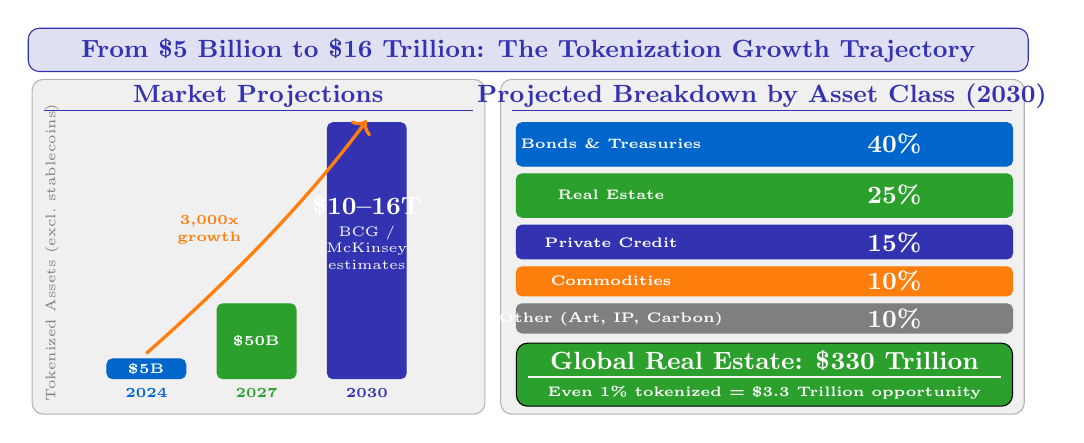
\begin{tikzpicture}
  % Header bar
  \draw[fill=mlpurple!15, draw=mlpurple, rounded corners=4pt] (0.0,4.5) rectangle (12.7,5.05);
  \node[font=\small\bfseries, mlpurple, align=center] at (6.35,4.77) {From \$5 Billion to \$16 Trillion: The Tokenization Growth Trajectory};

  % --- Left: Market Size Projections (bar chart) ---
  \draw[fill=lightgray, draw=midgray, rounded corners=4pt] (0.05,0.15) rectangle (5.8,4.4);
  \node[font=\small\bfseries, mlpurple, align=center] at (2.92,4.18) {Market Projections};
  \draw[mlpurple, thin] (0.2,4.0) -- (5.65,4.0);

  % Y-axis label
  \node[font=\tiny, mlgray, align=center, rotate=90] at (0.3,2.2) {Tokenized Assets (excl.\ stablecoins)};

  % Bar 1: 2024
  \draw[fill=mlblue, draw=mlblue, rounded corners=2pt] (1.0,0.6) rectangle (2.0,0.85);
  \node[font=\tiny\bfseries, white, align=center] at (1.5,0.72) {\$5B};
  \node[font=\tiny\bfseries, mlblue, align=center] at (1.5,0.42) {2024};

  % Bar 2: 2027
  \draw[fill=mlgreen, draw=mlgreen, rounded corners=2pt] (2.4,0.6) rectangle (3.4,1.55);
  \node[font=\tiny\bfseries, white, align=center] at (2.9,1.08) {\$50B};
  \node[font=\tiny\bfseries, mlgreen, align=center] at (2.9,0.42) {2027};

  % Bar 3: 2030
  \draw[fill=mlpurple, draw=mlpurple, rounded corners=2pt] (3.8,0.6) rectangle (4.8,3.85);
  \node[font=\small\bfseries, white, align=center] at (4.3,2.8) {\$10--16T};
  \node[font=\tiny, white, align=center] at (4.3,2.45) {BCG /};
  \node[font=\tiny, white, align=center] at (4.3,2.25) {McKinsey};
  \node[font=\tiny, white, align=center] at (4.3,2.05) {estimates};
  \node[font=\tiny\bfseries, mlpurple, align=center] at (4.3,0.42) {2030};

  % Growth arrow
  \draw[->, very thick, mlorange] (1.5,0.92) .. controls (2.5,1.8) and (3.5,2.8) .. (4.3,3.88);
  \node[font=\tiny\bfseries, mlorange, align=center] at (2.3,2.6) {3,000x};
  \node[font=\tiny\bfseries, mlorange, align=center] at (2.3,2.38) {growth};

  % --- Right: Breakdown by Asset Class ---
  \draw[fill=lightgray, draw=midgray, rounded corners=4pt] (6.0,0.15) rectangle (12.65,4.4);
  \node[font=\small\bfseries, mlpurple, align=center] at (9.32,4.18) {Projected Breakdown by Asset Class (2030)};
  \draw[mlpurple, thin] (6.15,4.0) -- (12.5,4.0);

  % Stacked bars / breakdown
  % Bonds: 40%
  \draw[fill=mlblue, draw=mlblue, rounded corners=2pt] (6.2,3.3) rectangle (12.5,3.85);
  \node[font=\tiny\bfseries, white, align=center] at (7.4,3.58) {Bonds \& Treasuries};
  \node[font=\small\bfseries, white, align=center] at (11.0,3.58) {40\%};

  % Real Estate: 25%
  \draw[fill=mlgreen, draw=mlgreen, rounded corners=2pt] (6.2,2.65) rectangle (12.5,3.2);
  \node[font=\tiny\bfseries, white, align=center] at (7.4,2.93) {Real Estate};
  \node[font=\small\bfseries, white, align=center] at (11.0,2.93) {25\%};

  % Private Credit: 15%
  \draw[fill=mlpurple, draw=mlpurple, rounded corners=2pt] (6.2,2.12) rectangle (12.5,2.55);
  \node[font=\tiny\bfseries, white, align=center] at (7.4,2.33) {Private Credit};
  \node[font=\small\bfseries, white, align=center] at (11.0,2.33) {15\%};

  % Commodities: 10%
  \draw[fill=mlorange, draw=mlorange, rounded corners=2pt] (6.2,1.65) rectangle (12.5,2.02);
  \node[font=\tiny\bfseries, white, align=center] at (7.4,1.84) {Commodities};
  \node[font=\small\bfseries, white, align=center] at (11.0,1.84) {10\%};

  % Other: 10%
  \draw[fill=mlgray, draw=mlgray, rounded corners=2pt] (6.2,1.18) rectangle (12.5,1.55);
  \node[font=\tiny\bfseries, white, align=center] at (7.4,1.36) {Other (Art, IP, Carbon)};
  \node[font=\small\bfseries, white, align=center] at (11.0,1.36) {10\%};

  % Key stat callout
  \draw[fill=mlgreen, rounded corners=4pt] (6.2,0.25) rectangle (12.5,1.05);
  \node[font=\small\bfseries, white, align=center] at (9.35,0.82) {Global Real Estate: \$330 Trillion};
  \draw[white, thin] (6.35,0.62) -- (12.35,0.62);
  \node[font=\tiny\bfseries, white, align=center] at (9.35,0.42) {Even 1\% tokenized = \$3.3 Trillion opportunity};
\end{tikzpicture}

\bottomnote{The RWA tokenization market is projected to grow from \$5B (2024) to \$10--16T by 2030 (BCG/McKinsey). Bonds and treasuries lead adoption (40\%), followed by real estate (25\%). Global real estate alone is \$330T -- just 1\% tokenized equals \$3.3T.}
\end{frame}

% Frame 10: Key Takeaways
\begin{frame}{Key Takeaways}
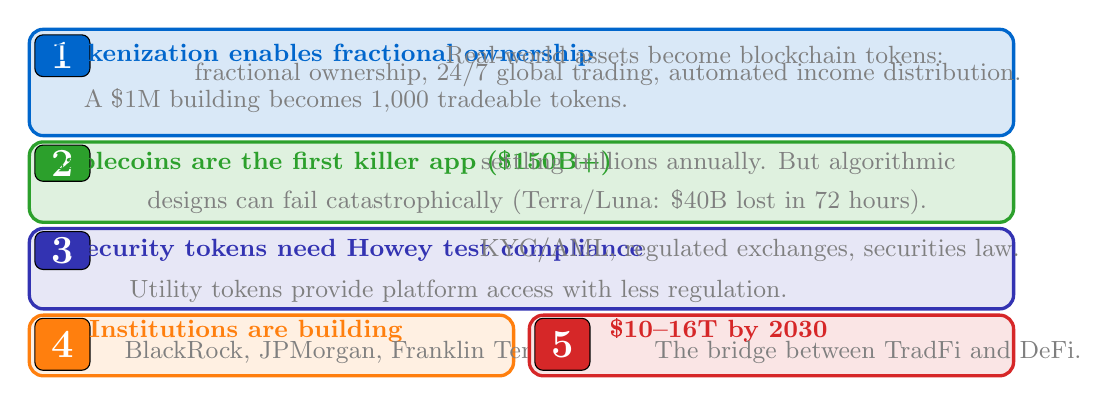
\begin{tikzpicture}
  % Box 1
  \draw[fill=mlblue!15, draw=mlblue, very thick, rounded corners=5pt] (0.05,3.2) rectangle (12.55,4.55);
  \draw[fill=mlblue, rounded corners=3pt] (0.12,3.95) rectangle (0.82,4.48);
  \node[font=\Large\bfseries, white, align=center] at (0.47,4.22) {1};
  \node[font=\small\bfseries, mlblue, align=center] at (3.8,4.22) {Tokenization enables fractional ownership};
  \node[font=\small, mlgray, align=center] at (8.5,4.22) {Real-world assets become blockchain tokens:};
  \node[font=\small, mlgray, align=center] at (7.4,3.98) {fractional ownership, 24/7 global trading, automated income distribution.};
  \node[font=\small, mlgray, align=center] at (4.2,3.65) {A \$1M building becomes 1,000 tradeable tokens.};

  % Box 2
  \draw[fill=mlgreen!15, draw=mlgreen, very thick, rounded corners=5pt] (0.05,2.1) rectangle (12.55,3.12);
  \draw[fill=mlgreen, rounded corners=3pt] (0.12,2.62) rectangle (0.82,3.08);
  \node[font=\Large\bfseries, white, align=center] at (0.47,2.85) {2};
  \node[font=\small\bfseries, mlgreen, align=center] at (3.8,2.85) {Stablecoins are the first killer app (\$150B+)};
  \node[font=\small, mlgray, align=center] at (8.8,2.85) {settling trillions annually. But algorithmic};
  \node[font=\small, mlgray, align=center] at (6.5,2.35) {designs can fail catastrophically (Terra/Luna: \$40B lost in 72 hours).};

  % Box 3
  \draw[fill=mlpurple!12, draw=mlpurple, very thick, rounded corners=5pt] (0.05,1.0) rectangle (12.55,2.02);
  \draw[fill=mlpurple, rounded corners=3pt] (0.12,1.5) rectangle (0.82,1.98);
  \node[font=\Large\bfseries, white, align=center] at (0.47,1.74) {3};
  \node[font=\small\bfseries, mlpurple, align=center] at (4.2,1.74) {Security tokens need Howey test compliance};
  \node[font=\small, mlgray, align=center] at (9.2,1.74) {KYC/AML, regulated exchanges, securities law.};
  \node[font=\small, mlgray, align=center] at (5.5,1.22) {Utility tokens provide platform access with less regulation.};

  % Box 4
  \draw[fill=mlorange!12, draw=mlorange, very thick, rounded corners=5pt] (0.05,0.15) rectangle (6.2,0.92);
  \draw[fill=mlorange, rounded corners=3pt] (0.12,0.22) rectangle (0.82,0.88);
  \node[font=\Large\bfseries, white, align=center] at (0.47,0.55) {4};
  \node[font=\small\bfseries, mlorange, align=center] at (2.8,0.72) {Institutions are building};
  \node[font=\small, mlgray, align=center] at (4.4,0.45) {BlackRock, JPMorgan, Franklin Templeton.};

  % Box 5
  \draw[fill=mlred!12, draw=mlred, very thick, rounded corners=5pt] (6.4,0.15) rectangle (12.55,0.92);
  \draw[fill=mlred, rounded corners=3pt] (6.47,0.22) rectangle (7.17,0.88);
  \node[font=\Large\bfseries, white, align=center] at (6.82,0.55) {5};
  \node[font=\small\bfseries, mlred, align=center] at (8.8,0.72) {\$10--16T by 2030};
  \node[font=\small, mlgray, align=center] at (10.7,0.45) {The bridge between TradFi and DeFi.};
\end{tikzpicture}

\vspace{0.1cm}
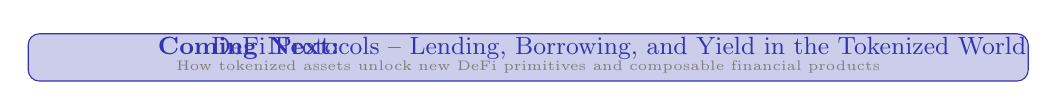
\begin{tikzpicture}
  \draw[fill=mllavender3, draw=mlpurple, rounded corners=4pt] (0,0) rectangle (12.7,0.6);
  \node[font=\small\bfseries, mlpurple] at (2.8,0.42) {Coming Next:};
  \node[font=\small, mlpurple] at (7.5,0.42) {DeFi Protocols -- Lending, Borrowing, and Yield in the Tokenized World};
  \node[font=\tiny, mlgray] at (6.35,0.18) {How tokenized assets unlock new DeFi primitives and composable financial products};
\end{tikzpicture}

\bottomnote{Tokenization is not a speculative promise -- it is actively being built by the world's largest institutions. The RWA market could reach \$10--16 trillion by 2030, forming the bridge between traditional finance and decentralized finance.}
\end{frame}

\end{document}
